\section{Building User-Applications with Konduit}

An added benefit of structured information is its potential for reuse: being able to integrate existing data, relieves users from creating it again. While a large part of the data is found online, when it comes to working with information, users still rely on the familiar environment of desktop-based applications. On the other hand, Web-based applications can only access Web data, and do not integrate well with desktop information.

Konduit \cite{Dragan2009b} offers a way of accessing structured Web data from the desktop, integrating it with existing desktop data and applications, and working with both in a unified way. It precedes the system for finding Web aliases for semantic resources from the desktop, presented in Chapter \ref{ch:sdwod}. 

The goal of Konduit was to allow the users to easily design their own personalised applications, customised to their needs and based on their workflows, without requiring prior knowledge of programming languages, or even semantics.
Our approach with Konduit is based on a combination of the visual programming paradigm and the idea of UNIX pipes, and allows the casual users to build simple programs in order to perform and automate everyday tasks on RDF data. In other words, it is visual programming for RDF. 

\subsection{Components and Workflows}
\label{sec:konduit_components_and_workflows}

Konduit provides a collection of useful components ready for immediate use. The components offer individual units of functionality and are represented visually as blocks. They are connected through input and output slots, and in this way the flow of the program is defined. In order to keep simple the task of connecting components, the only data that flows through the workflow is RDF. This condition ensures that each component always fulfils the minimal requirement for dealing with its input. Obviously, components may be specialised with respect to the actual vocabulary on which they can operate and will decide at runtime if and how they deal with the incoming RDF. By neither allowing different kinds of data (e.g., text, numbers, lists, images, etc.), nor typing the RDF data with respect to the vocabularies they use, we stay very close to the original UNIX pipes concept, where data is always an untyped stream of bytes, and where it is up to each process or program how to handle it. 

The architecture of Konduit is modular, each component is realised as a plugin which can be independently installed or removed. We expect that new plugins will be developed and shared by external power users, as the need for them arises. 
Formally, a component is defined by the following parameters:
$$
Component = (I, O, P, F )
$$
\begin{itemize}
 \item a set of RDF input slots $I$,
 \item a set of RDF output slots $O$, 
 \item a set of parameters $P$ which allow for user input in the workflow, 
 \item a function $F$, which works on the input $I$ and generates the output $O$.
\end{itemize}
The parameters $P$ influence the behaviour of $F$.

The number of input and output slots is not fixed and can be 0 or more. Depending on the number of slots, components can be grouped in three categories: sources, sinks, and ordinary components. Sources are components that do not have any inputs. They supply the workflow with data. There is always at least one source at the start of any workflow. Because data graphs can be merged, there can be more than one source for any workflow. Typical examples of sources are connectors to RDF stores, file (URL) input components, or converters from other, non-RDF formats. Sinks are components that do not have any outputs. They represent the final point(s) of any workflow. Examples of sink components are application adaptors, serialisers (file output components) and visualisers. In Konduit, workflows are activated from a sink component, usually by clicking on an activation button.

Several connected components make up a workflow, which is defined by specifying
$$
Workflow = (C, f) , where f: inputs(C) \rightarrow outputs(C) \cup \{~nil~\}
$$
\begin{itemize}
 \item a set of components $C$,
 \item a function $f$ defined from the set of all the inputs of the components of $C$ to the set of all the outputs of the components of $C$ and the $nil$ output.
\end{itemize}
The function $f$ shows how the components of $C$ are connected. The inputs that are not connected have a $nil$ value of $f$; the outputs that do not represent a value of $f$ are not connected.

Workflows can be saved and reused. Saving a workflow implies saving all the components that have at least one connection to it, as well as their existing connections, parameters and layout. There is no restriction that the components should be completely connected, so there can be input or output slots that remain open. A saved workflow can be reopened and modified by adding to it or removing components, or by changing connection or parameters and thus obtaining different workflows with minimum effort.

An important aspect of Konduit is directly tied to the fact that all inputs and outputs are RDF graphs. As a result, any workflow can itself become a component, meaning that workflows can be built recursively. In this way, it is possible to create specialised components, which we call black boxes, based on the combination of other components. The blackboxes are added to the existing library for reuse. An example of saved workflows and blackboxes is shown in Figure \ref{fig:discography_generator}. The workflow is taken from \url{http://smile.deri.ie/konduit/discography}, where an entire example use case is presented.

\begin{figure}[!ht]
 \centering
 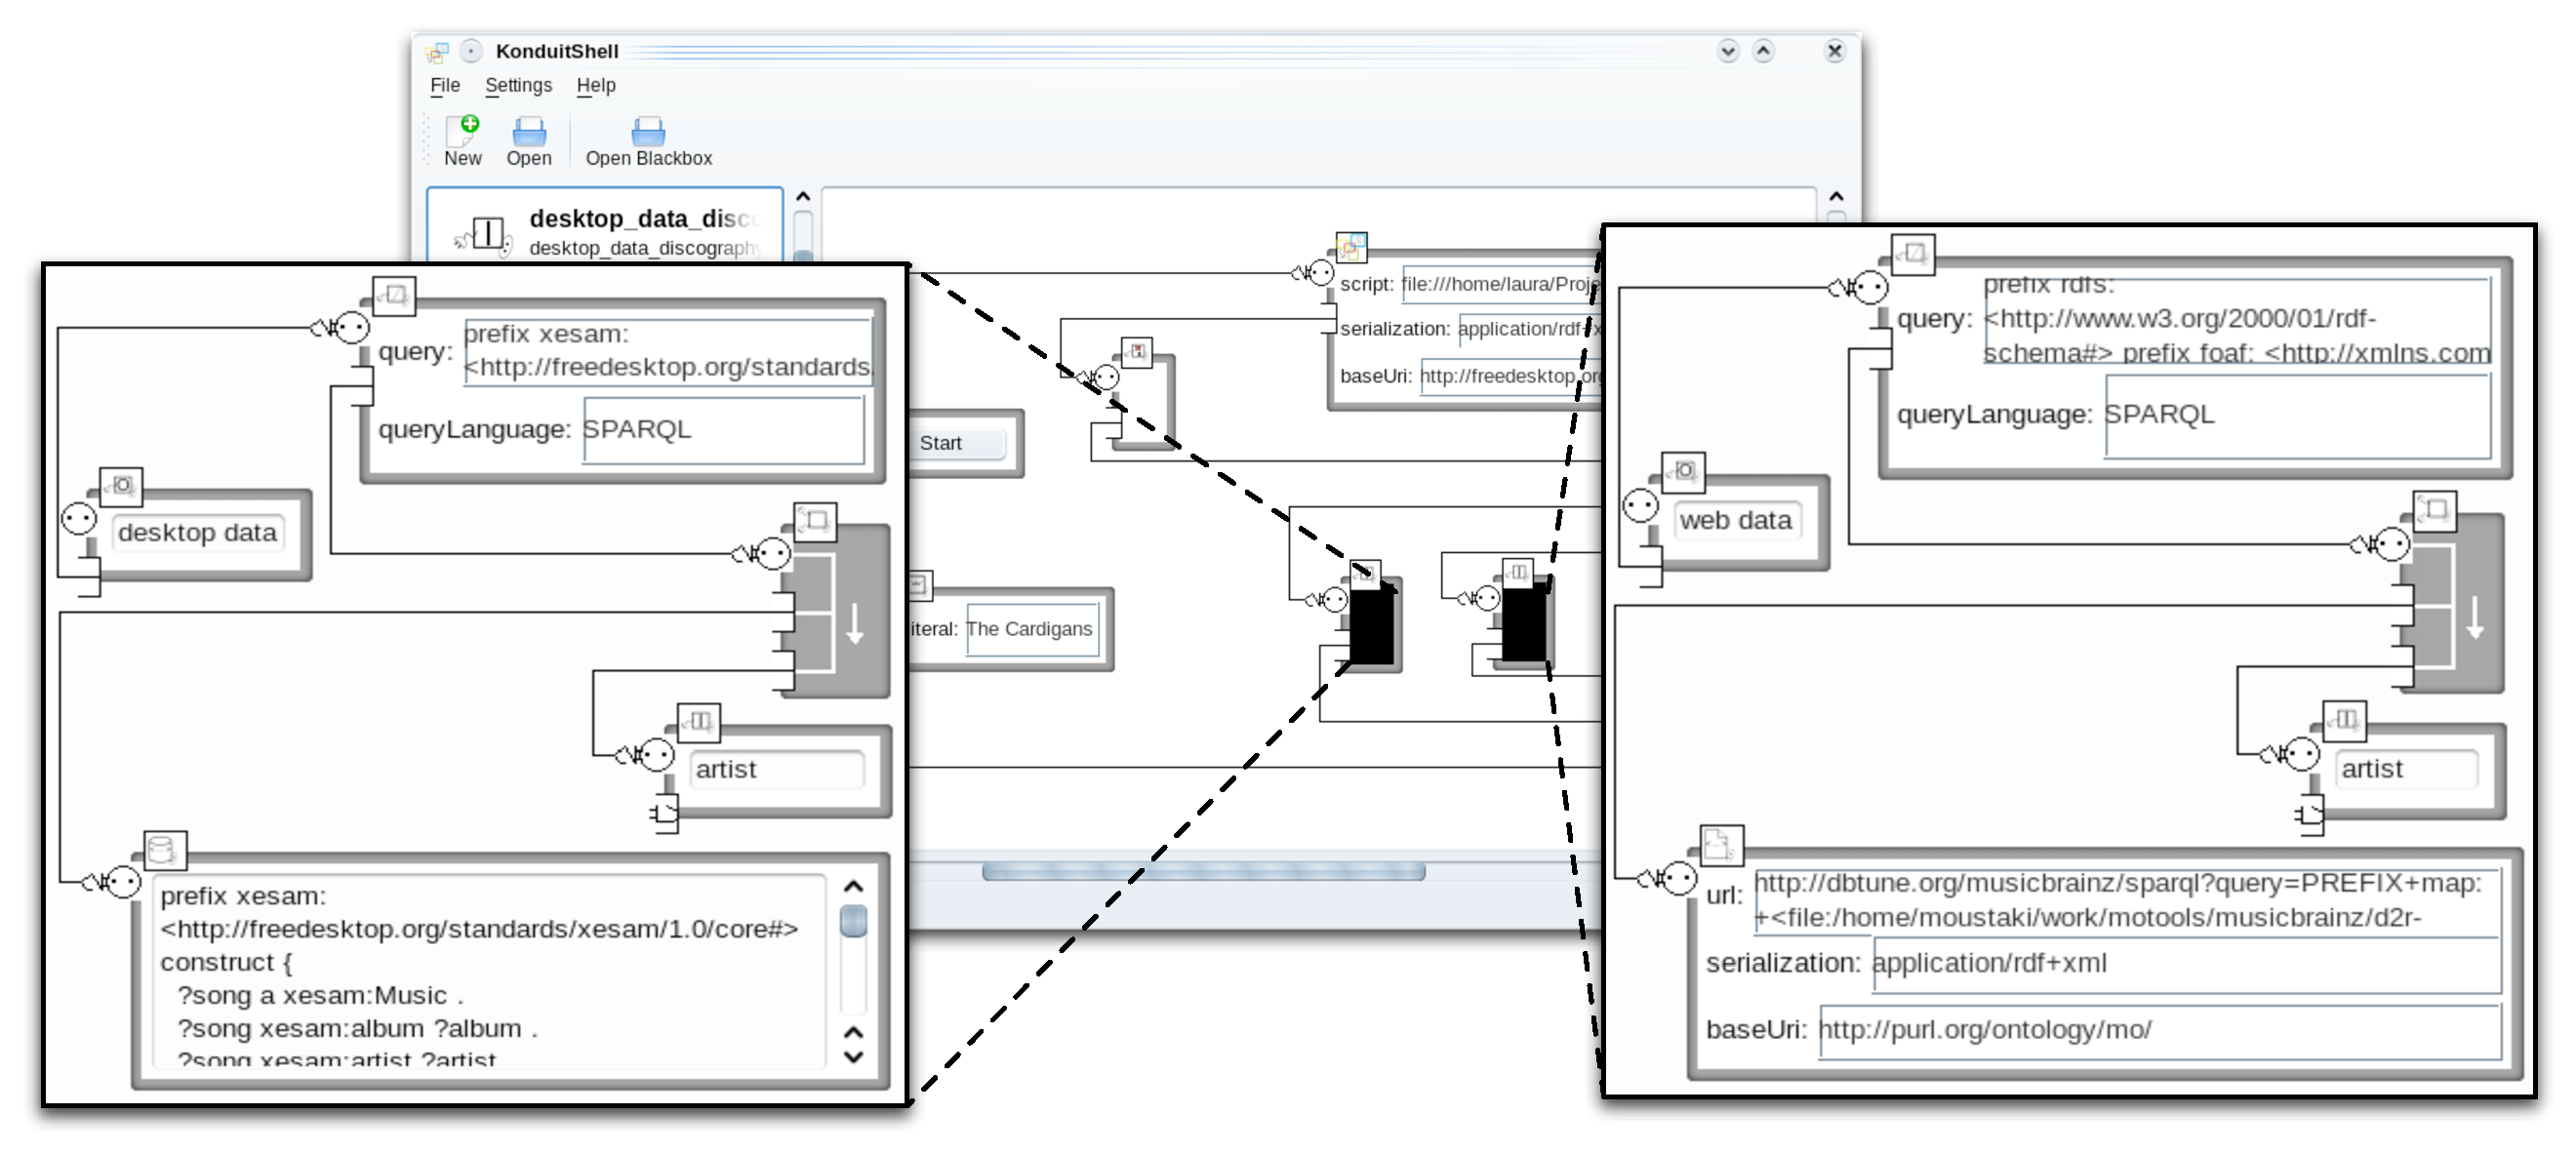
\includegraphics[width=1.0\linewidth]{chapters/core/img/discography}
 \caption{The entire discography generator workflow.}
 \label{fig:discography_generator}
\end{figure}

\cite{Dragan2009b} describes in more detail the different types of sources, sinks, and ordinary component types, as well as the blackbox mechanism. 
Some of the basic components available for Konduit require previous knowledge of writing SPARQL queries. Since the queries can influence the performance of the entire workflow, we recognise the need for a smart query editor that is suitable for naive users. \cite{Ambrus2010} describes the means for making Konduit more user friendly, by adding a smart wizard with suggestions and SPARQL autocompletion. 
